\documentclass{utue} %utue.cls required for Uni Tuebingen corporate design

% Values for title generation
\title{Controlling Phasor Noise Artifacts}
\author{Jonathan Lang}
\date{\today}

% Subtitle is optional. It represents what kind of work you did.
\subtitle{Research Project}

\begin{document}

% You can place a teaser as follows. (Otherwise, just uncomment the following part)
%\teaser{
%    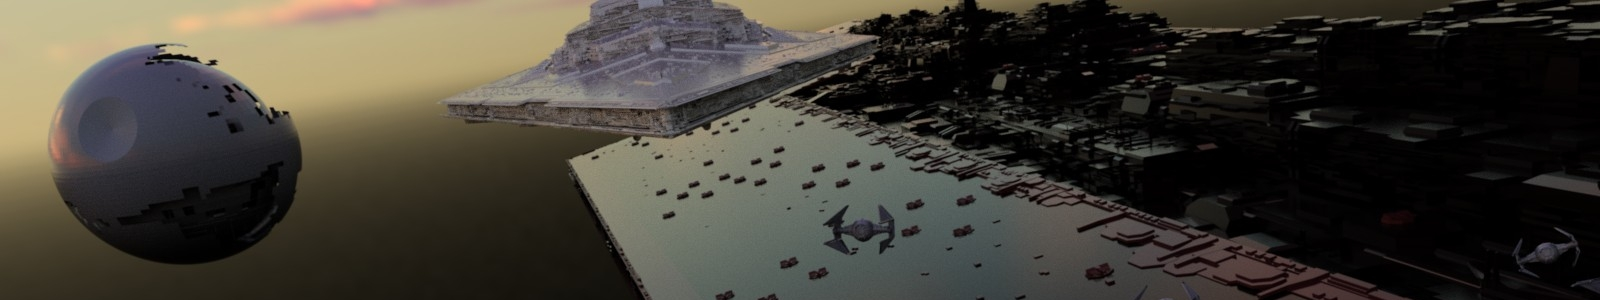
\includegraphics[width=\textwidth]{images/teaser.jpg}
%    \caption{\label{fig:teaser}You can place a teaser here.}
%}     

% Creates title of document and additional title page.
\maketitle 
 
\section*{Abstract}  
  
\section{Introduction}   
To keep up with the shorter development cycles of the current times more work has to be done in shorter time. The tools with which this is achieved are optimization of workflows as well as automation. While even the automation of repetitive tasks can be challenging, automating creative tasks like content creation is even more so. This is where noise algorithms provide assistance. They provide a way to generate non-repeating patterns over potentially infinite space at low memory and computational cost. Using these patterns two influence different aspect of the content, anything form additional detail on surfaces up to the layout of whole worlds can be generated automatically. The generated patterns are as varied as the algorithms itself. The different algorithms also provide different levels of influence over the produced pattern. Additional Parameters to tune the generated pattern are of course desirable, as a richer set of patterns will be applicable for more situations, therefore offering further automation opportunities.


\section{Related Work} 



\bibliographystyle{alpha}
\bibliography{bibliography}

\end{document}

